\documentclass[10pt,UTF8]{ctexart}


\usepackage[margin=2cm,a4paper]{geometry}
%\usepackage[left=0.75in,top=0.6in,right=0.75in,bottom=1.0in,a4paper]{geometry}

\setmainfont{Caladea}
%% 也可以選用其它字庫:
% \setCJKmainfont[%
%   ItalicFont=AR PL KaitiM GB,
%   BoldFont=Noto Sans CJK SC,
% ]{Noto Serif CJK SC}
% setCJKsansfont{Noto Sans CJK SC}
% \renewcommand{\kaishu}{\CJKfontspec{AR PL KaitiM GB}}

% 繁體中文
\setCJKmainfont[Path=fonts/ ]{NotoSansTC-Medium.otf}

\usepackage{minted}
\usepackage[breaklinks]{hyperref}

% Picture
% 導言區的此三行無變化
\usepackage{graphicx}
\usepackage{float} 
\usepackage{subfigure}
% 以下是新增的自定義格式更改
\usepackage[]{caption2} %新增調用的宏包
\renewcommand{\figurename}{Fig.} %重定義編號前綴詞
\renewcommand{\captionlabeldelim}{.~} %重定義分隔符
 %\roman 是羅馬數字編號,\alph是默認的字母編號,\arabic是阿拉伯數字編號,可按需替換下一行的相應位置
\renewcommand{\thesubfigure}{(\roman{subfigure})}%此外,還可設置圖編號顯示格式,加括號或者不加括號
\makeatletter \renewcommand{\@thesubfigure}{\thesubfigure \space}%子圖編號與名稱的間隔設置
\renewcommand{\p@subfigure}{} \makeatother

% Math
\usepackage {mathtools}
\usepackage{amssymb}

% Code
\usepackage{listings}
\usepackage{xcolor}
\lstset{
    % backgroundcolor=\color{red!50!green!50!blue!50},
    % 程式碼塊背景色為淺灰色
    rulesepcolor= \color{gray}, % 程式碼塊邊框顏色
    breaklines=true,  % 程式碼過長則換行
    numbers=left, % 行號在左側顯示
    numberstyle= \small,% 行號字型
    % eywordstyle= \color{red,% 關鍵字顏色
    commentstyle=\color{gray}, % 註釋顏色
    frame=shadowbox % 用方框框住程式碼塊
    }

\usepackage{hyperref}

\title{算法分析和複雜性理論}
\author{干皓丞,2101212850, 信息工程學院}

\begin{document}
\maketitle


\section{作業目標與章節摘要}

1. LeetCode 16. 3Sum Closest 整數反轉

2. LeetCode 17. Letter Combinations of a Phone Number 電話號碼的字母組合

3. LeetCode 19. Remove Nth Node From End of List 刪除鍊錶的倒數第 N 個結點


\section{作業內容概述}

作業可以從 GitHub 下的 kancheng/kan-cs-report-in-2022 專案找到,作業程式碼與文件目錄為 kan-cs-report-in-2022/AATCC/lab-report/w3。實際執行的環境與實驗設備為 Google 的 Colab 、MacBook Pro (Retina, 15-inch, Mid 2014) 、 Acer Aspire R7 與 HP Victus (Nvidia GeForce RTX 3060)。

本作業 GitHub 專案為 kancheng/kan-cs-report-in-2022 下的 AATCC` 的目錄。程式碼可以從 code 目錄下可以找到 *.pynb,內容包含上次課堂練習、LeetCode 範例思路整理與作業。

https://github.com/kancheng/kan-cs-report-in-2022/tree/main/AATCC

\begin{figure}[H]
\centering 

\includegraphics[width=0.30\textwidth]{aatccqr.png} 
\caption{作業專案位置}
\label{Test}
\end{figure}


1. LeetCode : https://leetcode.com/

2. LeetCode CN : https://leetcode-cn.com/

3. OnlineGDB : https://www.onlinegdb.com/ 

LeetCode 的平台部分, CN 的平台有針對簡體中文使用者進行處理,包含中英文切換等功能。OnlineGDB 則可線上進行簡易的環境測試,其程式碼涵蓋 C, C++, C\#, Java, Python, JS, Rust, Go。

\newpage

\section{LeetCode 16. 3Sum Closest 整數反轉}

\subsection{LeetCode 16. 題目}

Given an integer array nums of length n and an integer target, find three integers in nums such that the sum is closest to target.

Return the sum of the three integers.

You may assume that each input would have exactly one solution.

給你一個長度為 n 的整數數組 nums 和 一個目標值 target。請你從 nums 中選出三個整數,使它們的和與 target 最接近。

返回這三個數的和。

假定每組輸入只存在恰好一個解。

Example 1:
\begin{lstlisting}[language={python}]
Input: nums = [-1,2,1,-4], target = 1
Output: 2
Explanation: The sum that is closest to the target is 2. (-1 + 2 + 1 = 2).
\end{lstlisting}

Example 2:
\begin{lstlisting}[language={python}]
Input: nums = [0,0,0], target = 1
Output: 0
\end{lstlisting}

Constraints:

- 3 <= nums.length <= 1000

- -1000 <= nums[i] <= 1000

- $-10^4$ <= target <= $10^4$

\subsection{LeetCode 16. 思路總結}

這一題的解法是用兩個指針夾逼的方法。先對數組進行排序,i 從頭開始往後面掃。這裡同樣需要注意數組中存在多個重複數字的問題。具體處理方法很多,可以用 map 計數去重。這裡筆者簡單的處理,i 在循環的時候和前一個數進行比較,如果相等,i 繼續往後移,直到移到下一個和前一個數字不同的位置。 j,k 兩個指針開始一前一後夾逼。 j 為 i 的下一個數字,k 為數組最後一個數字,由於經過排序,所以 k 的數字最大。 j 往後移動,k 往前移動,逐漸夾逼出最接近 target 的值。

這道題還可以用暴力解法,三層循環找到距離 target 最近的組合。

\subsection{LeetCode 16. Code 範例}

LeetCode 16. Python 

\begin{lstlisting}[language={python}]
from typing import List
class Solution:
    def threeSumClosest(self, nums: List[int], target: int) -> int:
        n = len(nums)
        nums.sort()
        re_min = 0 #存储当前最小的差值
        for i in range(n):
            low = i+1
            high = n-1
            while low < high:
                three_sum = nums[i] + nums[low] + nums[high]
                x = target - three_sum #当前三数的差值
                if re_min == 0:
                    re_min = abs(x)
                    sum_min = three_sum #sum_min为当前最接近的和
                if abs(x) < re_min:
                    re_min = abs(x)
                    sum_min = three_sum
                if three_sum == target:
                    return target
                elif three_sum < target:
                    low += 1
                else:
                    high -= 1
        return sum_min
\end{lstlisting}

\subsection{LeetCode 16. 結果}

\begin{figure}[H]
\centering 
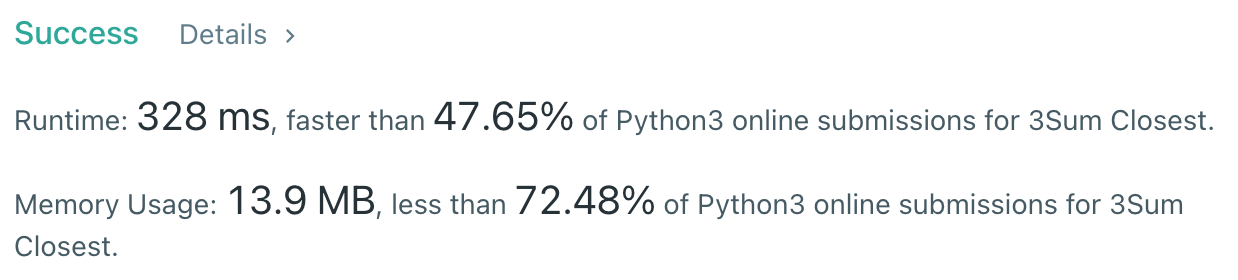
\includegraphics[width=0.80\textwidth]{lc-16-o.png} 
\caption{LeetCode 16 結果}
\label{Test}
\end{figure}


\newpage

\section{LeetCode 17. Letter Combinations of a Phone Number 電話號碼的字母組合}

\subsection{LeetCode 17. 題目}

Given a string containing digits from 2-9 inclusive, return all possible letter combinations that the number could represent. Return the answer in any order.

A mapping of digit to letters (just like on the telephone buttons) is given below. Note that 1 does not map to any letters.

給定一個僅包含數字 2-9 的字符串,返回所有它能表示的字母組合。答案可以按 任意順序 返回。

給出數字到字母的映射如下(與電話按鍵相同)。注意 1 不對應任何字母。

\begin{figure}[H]
\centering 
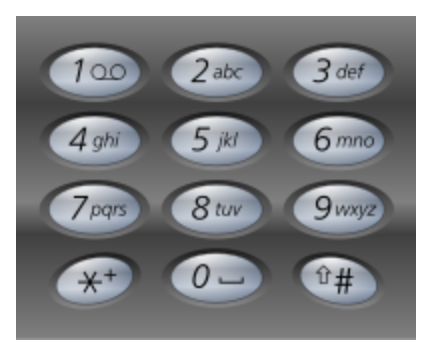
\includegraphics[width=0.80\textwidth]{lc-16-p-example.png} 
\caption{Example 1}
\label{Test}
\end{figure}

Example 1:
\begin{lstlisting}[language={python}]
Input: digits = "23"
Output: ["ad","ae","af","bd","be","bf","cd","ce","cf"]
\end{lstlisting}

Example 2:
\begin{lstlisting}[language={python}]
Input: digits = ""
Output: []
\end{lstlisting}

Example 3:
\begin{lstlisting}[language={python}]
Input: digits = "2"
Output: ["a","b","c"]
\end{lstlisting}


Constraints:

- 0 <= digits.length <= 4

- digits[i] is a digit in the range ['2', '9'].(digits[i] 是范圍 ['2', '9'] 的一個數字。)

\subsection{LeetCode 17. 思路總結}

DFS 遞歸深搜

Reference : https://www.bilibili.com/video/BV1cy4y167mM/

\begin{lstlisting}[language={python}]
class Solution(object):
    def letterCombinations(self, digits):
        """
        动态规划
        dp[i]: 前i个字母的所有组合
        由于dp[i]只与dp[i-1]有关,可以使用变量代替列表存储降低空间复杂度
        :type digits: str
        :rtype: List[str]
        """
        if not digits:
            return []
        d = {'2': 'abc', '3': 'def', '4': 'ghi', '5': 'jkl',
             '6': 'mno', '7': 'pqrs', '8': 'tuv', '9': 'wxyz'}
        n = len(digits)
        dp = [[] for _ in range(n)]
        dp[0] = [x for x in d[digits[0]]]
        for i in range(1, n):
            dp[i] = [x + y for x in dp[i - 1] for y in d[digits[i]]]
        return dp[-1]

    def letterCombinations2(self, digits):
        """
        使用变量代替上面的列表
        降低空间复杂度
        :type digits: str
        :rtype: List[str]
        """
        if not digits:
            return []
        d = {'2': 'abc', '3': 'def', '4': 'ghi', '5': 'jkl',
             '6': 'mno', '7': 'pqrs', '8': 'tuv', '9': 'wxyz'}
        n = len(digits)
        res = ['']
        for i in range(n):
            res = [x + y for x in res for y in d[digits[i]]]
        return res

    def letterCombinations3(self, digits):
        """
        递归
        :param digits:
        :return:
        """
        d = {'2': 'abc', '3': 'def', '4': 'ghi', '5': 'jkl',
             '6': 'mno', '7': 'pqrs', '8': 'tuv', '9': 'wxyz'}
        if not digits:
            return []
        if len(digits) == 1:
            return [x for x in d[digits[0]]]
        return [x + y for x in d[digits[0]] for y in self.letterCombinations3(digits[1:])]
\end{lstlisting}

\subsection{LeetCode 17. Code 範例}

\begin{lstlisting}[language={python}]
class Solution(object):
    def letterCombinations(self, digits):
        if not digits:
            return []
        d = {'2': 'abc', '3': 'def', '4': 'ghi', '5': 'jkl',
             '6': 'mno', '7': 'pqrs', '8': 'tuv', '9': 'wxyz'}
        n = len(digits)
        dp = [[] for _ in range(n)]
        dp[0] = [x for x in d[digits[0]]]
        for i in range(1, n):
            dp[i] = [x + y for x in dp[i - 1] for y in d[digits[i]]]
        return dp[-1]
\end{lstlisting}

\subsection{LeetCode 17. 結果}

\begin{figure}[H]
\centering 
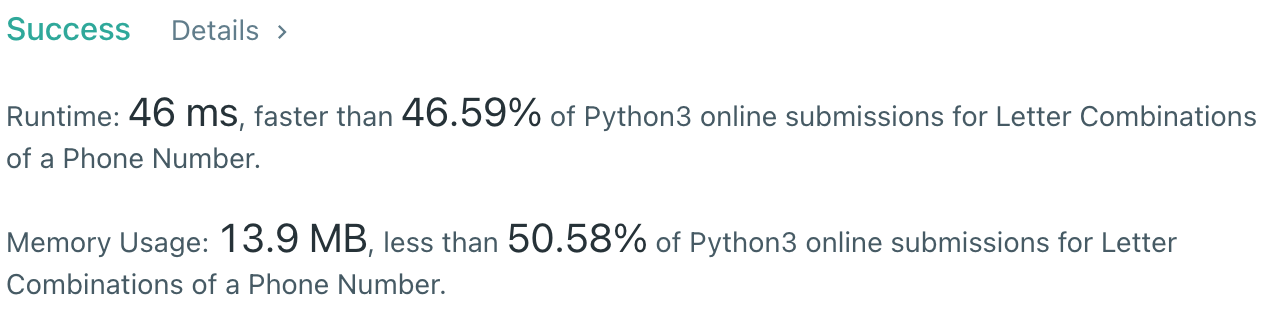
\includegraphics[width=0.80\textwidth]{lc-17-o.png} 
\caption{LeetCode 17 結果}
\label{Test}
\end{figure}


\newpage

\section{LeetCode 19. Remove Nth Node From End of List 刪除鍊錶的倒數第 N 個結點}

\subsection{LeetCode 19. 題目}

Given the head of a linked list, remove the $n^{th}$ node from the end of the list and return its head.

給你一個鍊錶,刪除鍊錶的倒數第 n 個結點,並且返回鍊錶的頭結點。

\begin{figure}[H]
\centering 
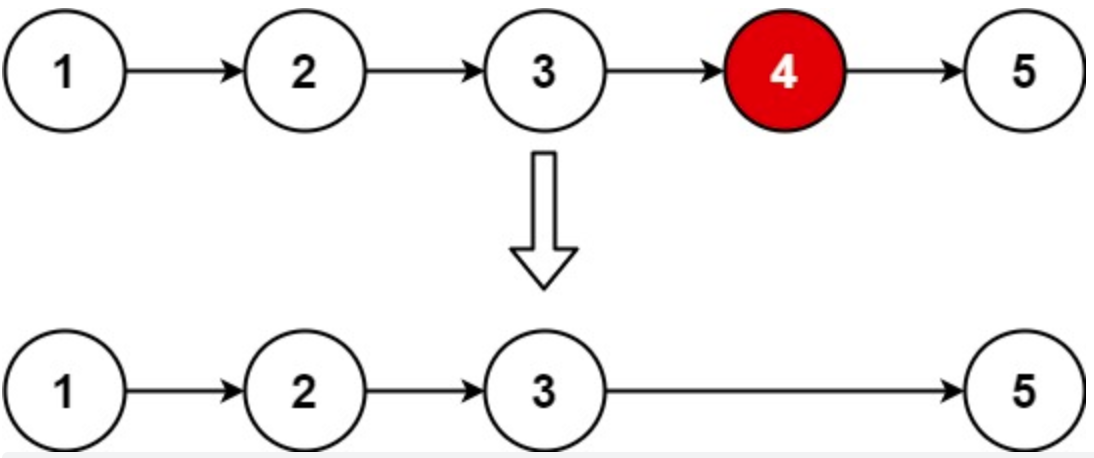
\includegraphics[width=0.80\textwidth]{lc-19-p-example.png} 
\caption{Example 1}
\label{Test}
\end{figure}

Example 1:
\begin{lstlisting}[language={python}]
Input: head = [1,2,3,4,5], n = 2
Output: [1,2,3,5]
\end{lstlisting}

Example 2:
\begin{lstlisting}[language={python}]
Input: head = [1], n = 1
Output: []
\end{lstlisting}

Example 3:
\begin{lstlisting}[language={python}]
Input: head = [1,2], n = 1
Output: [1]
\end{lstlisting}

Constraints:

1. The number of nodes in the list is sz.(鍊錶中結點的數目為 sz)

2. 1 <= sz <= 30

3. 0 <= Node.val <= 100

4. 1 <= n <= sz

Follow up: Could you do this in one pass?(你能嘗試使用一趟掃描實現嗎?)

\subsection{LeetCode 19. 思路總結}

1. 先循環一次拿到鍊錶的總長度,然後循環到要刪除的結點的前一個結點開始刪除操作。需要注意的一個特例是,有可能要刪除頭結點,要單獨處理。

2. 這道題有一種特別簡單的解法。設置 2 個指針,一個指針距離前一個指針 n 個距離。同時移動 2 個指針,2 個指針都移動相同的距離。當一個指針移動到了終點,那麼前一個指針就是倒數第 n 個節點了

Reference : https://stackoverflow.com/questions/61610160/remove-nth-node-from-end-of-listleetcode-python

\subsection{LeetCode 19. Code 範例}

\begin{lstlisting}[language={python}]
"""
class Solution:
    def removeNthFromEnd(self, head: ListNode, n: int) -> ListNode:
        head_dummy = ListNode()
        head_dummy.next = head

        slow, fast = head_dummy, head_dummy
        while(n!=0): # fast先往前走n步
            fast = fast.next
            n -= 1
        while(fast.next!=None):
            slow = slow.next
            fast = fast.next
        # fast 走到結尾後,slow 的下一個節點為倒數第N個節點
        slow.next = slow.next.next # 刪除
        return head_dummy.next
"""
class Solution:
    def removeNthFromEnd(self, head, n):
        fast = slow = head
        for _ in range(n):
            fast = fast.next
        if not fast:
            return head.next
        while fast.next:
            fast = fast.next
            slow = slow.next
        slow.next = slow.next.next
        return head
\end{lstlisting}

\subsection{LeetCode 19. 結果}

\begin{figure}[H]
\centering 
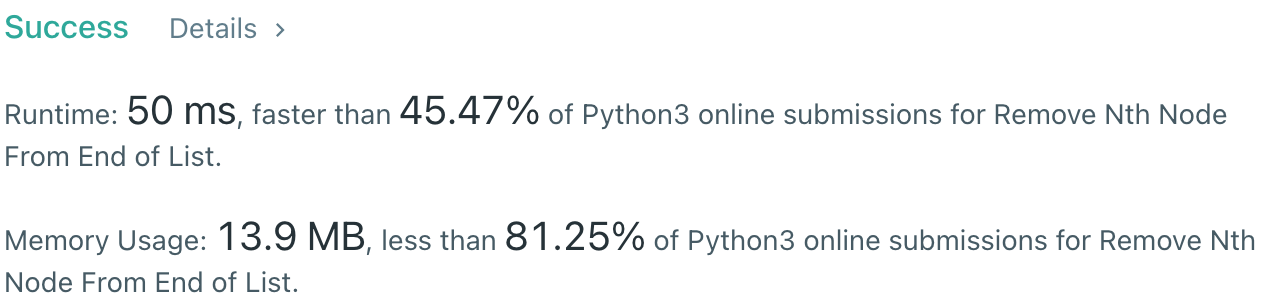
\includegraphics[width=0.80\textwidth]{lc-19-o.png} 
\caption{LeetCode 19 結果}
\label{Test}
\end{figure}




%\section{附錄}

% 數學意義說明

% $$\min \limits_{G}\max \limits_{D}{V_I(D,\ G)=V(D,G)-\lambda L_I(G,Q)}$$

%	\begin{lstlisting}[language={python}]

%	\end{lstlisting}

%\begin{enumerate}
%\item Y
%\item A
%\end{enumerate}

% \newpage

\clearpage

\end{document}